\section{Theoretical Background}\label{body_theoretical_background}
This chapter serves as a reference for the theoretical background necessary to understand the insights gained in the following experimental chapters.
Section \ref{theoretical_classification} discusses classification models used to train on the extended dataset resulting from the generative augmentation process. In it, \textit{Neural Networks} (NNs) for image classification are introduced and the baselines for later comparisons are examined.
Sections \ref{theoretical_da} and \ref{theoretical_gda} establish the foundation for data augmentation and generative data augmentation.
Following sections \ref{theoretical_gan}, \ref{theoretical_dcgan}, \ref{theoretical_cgan}, and \ref{theoretical_madgan} provide theoretical knowledge necessary to understand the GAN architectures and their differences. The narrative follows their increasing complexity, starting from vanilla GANs, moving through deep convolutional GANs and conditional GANs, before diving into the background of multi-agent diverse GANs.
The final section (\ref{theoretical_image_scores}) explains the theory behind the Inception Score and Fréchet Inception Distance, concluding with an examination of the state-of-the-art \textit{InceptionV3} model used to compute them.
% ########################################################################################################
% # START: IMAGE CLASSIFICATION MODELS
% ########################################################################################################
\subsection{Image Classification Models}\label{theoretical_classification}
\subsubsection{Neural Networks for Classification}
Convolutional Neural Networks (CNNs) have become the dominant architecture for image classification tasks due to their inherent ability to automatically learn hierarchical features from raw pixel data. At their core, CNNs are build up by a sequence of convolutional-, pooling- and fully connected layers to extract hierarchical features, and funneling the information, typically into the \(N\) classes defined by the training data. Convolutional layers employ learnable filters to detect local patterns in the two-dimensional information - two dimensional in the case of images specifically. Pooling layers reduce the spatial dimensions to small translations. Fully connected layers then map the extracted information into class probabilities, utilizing the \textit{Softmax} activation function. The afore mentioned layers are discussed in greater detail, in the following subsections.

\vspace{1em}

\textbf{Convolutional Layers}\label{theoretical_classification_conv_layers}
TODO: here is a nice place for a ref to \cite{Dumoulin2016TransposedConv}
These layers compute the output from the local regions of the input. Let $(r \times c)$ be the two-dimensional input, e.g., a grayscale image, where $r$ represents the X-coordinate and $c$ the Y-coordinate of a pixel. Thus, $r \cdot c$ denotes the size of the image. Furthermore, let $(a \times b)$ be a filter with kernel size $a \cdot b$, where the filter is smaller than the input. This filter is moved from the top-left to the bottom-right over the input.

In each iteration, the dot product between the respective coefficients of the input region and the coefficients of the filter is computed. This dot product is then processed by the activation function $g$, which determines how much of the feature is present. If the activation function is ReLU, for example, only positive values are retained, meaning negative responses are set to zero. The result is written to the subsequent layer.

The stride determines how far the filter is moved after each operation. For a stride of $s = 1$, the filter can be placed in $(r - a + 1)$ positions along the height and $(c - b + 1)$ positions along the width, leading to an output size of $(r - a + 1) \times (c - b + 1)$. In general, the output size in the two-dimensional case is given by:
\[
\left( \frac{r - a + s}{s} \right) \times \left( \frac{c - b + s}{s} \right).
\]
%TODO: point to the right figure
An image of this process can be found in Figure X in the Appendix (7). This image shows an input of size $[10 \times 10]$ and a filter of size $[3 \times 3]$. With a stride of $s = 1$, the resulting layer has a size of $[8 \times 8]$ (computed as $\left(10 - 3 + 1\right) \times \left(10 - 3 + 1\right)$).

The stride of the filter can also be greater than $1$. Additionally, there is the option to apply padding to the image. There are different ways to implement padding. When padding of size $p$ is applied, the output size for a square input and filter is calculated as follows:
\[
\textbf{Output size} = \left\lfloor \frac{r - a + 2p}{s} \right\rfloor + 1
\]
where $\lfloor \cdot \rfloor$ denotes the floor function, which ensures that the output size is an integer.

\vspace{1em}

\textbf{Pooling Layers}\label{theoretical_classification_pooling_layers}
A pooling layer compresses the data along the spatial axes to reduce its dimensionality. Similar to the convolutional layer, a pooling layer uses a filter that moves by the stride value. However, instead of summing the covered elements, the pooling operation applies the Max operator, selecting the maximum value within the filter's region.

For example, starting with an input of size $[32 \times 32 \times 10]$, applying a pooling operation with a $[2 \times 2]$ filter and a stride of 2 results in an output size of $[16 \times 16 \times 10]$. This operation reduces the spatial dimensions by half while keeping the depth unchanged.

Max pooling helps retain the most important features, providing some invariance to small translations or distortions in the input, which is crucial for tasks like object recognition in convolutional neural networks (CNNs).


\vspace{1em}

\textbf{Fully-Connected Layers}\label{theoretical_classification_fully_connected_layers}
Fully-Connected (FC), also called \textit{Dense} layer, typically computes the scores for the respective classes. In the case of ten classes, the result is a volume of size $[1 \times 1 \times 10]$\footnote{Typically, the output from the layer before the FC one is "flattened" into a one-dimensional vector, preserving all information but removing spatial structure. For example, a $[2 \times 2]$ layer would become a vector of size $[1 \times 4]$.}. By this stage, all spatial information has been transformed, leaving a quasi-one-dimensional vector containing the ten class scores for the CIFAR-10 dataset.

In a FC layer, each input is connected to each output, meaning every neuron in the previous layer is connected to each neuron in the FC layer. The output is the weighted sum of all inputs, followed by an activation function, leading to the final classification scores that represent the likelihood of the input belonging to each class. The spatial dimensions are collapsed into a single vector of class scores, which are then used for classification.

\textbf{Batch Normalization Layers}\label{theoretical_classification_batchnorm_layers}
With their introduction in "\textit{Batch Normalization: Accelerating Deep Network Training by Reducing Internal Covariate Shift}" by Ioffe et al. \cite{ioffe2015batchnormalizationacceleratingdeep}, Batch Normalization (batchnorm) is an integreal part of convolutional networks. These layers normalize the inputs to subsequent layers and theirby stability the distribution of activations throughout the training process. This reduces the internal covariate shift, allowing for higher learning rates and faster convergence. By normalization of activation, batchnorm helps prevent gradients from vanishing or exploding. Additionally, it can provide regularization benefits and eliminate the need for Dropout, in some cases. With the afore mentioned benefits, batchnorm layers are particularily beneficial for deep learning networks with many layers.


\textbf{Typical Activation Functions for CNNs}

\begin{itemize}
    \item \textbf{ReLU (Rectified Linear Unit)}: \label{theoretical_activations_relu}
    \begin{equation}
    g(x) = \max(0, x)
    \end{equation}
    ReLU is the most widely used activation function in CNNs. It introduces non-linearity while maintaining efficiency by outputting zero for negative values and passing positive values unchanged.

    \item \textbf{Leaky ReLU}: \label{theoretical_activations_leakyrelu}
    \begin{equation}
        f(x) =
        \begin{cases}
        0 \quad \text{if } x < 0 \\
        x \quad \text{otherwise}
        \end{cases}
    \end{equation}
    A variant of ReLU, Leaky ReLU allows small negative values to flow through, addressing the "dying ReLU" problem where neurons can become inactive.

    \item \textbf{Sigmoid (Logistic)}:  \label{theoretical_activations_sigmoid}
    \begin{equation}
        g(x) = \frac{1}{1 + e^{-x}}
    \end{equation}
    The sigmoid function squashes values between 0 and 1, commonly used for binary classification tasks. However, it can suffer from vanishing gradients for very large or small inputs.

    \item \textbf{Tanh (Hyperbolic Tangent)}:  \label{theoretical_activations_tanh}
    \begin{equation}
        g(x) = \frac{2}{1 + e^{-2x}} - 1
    \end{equation}
    Tanh outputs values between -1 and 1 and is similar to the sigmoid but with a wider output range, making it more effective in many scenarios compared to sigmoid.

    \item \textbf{Softmax}: \label{theoretical_activations_softmax}
    \begin{equation}
        g(x_i) = \frac{e^{x_i}}{\sum_{j} e^{x_j}}
    \end{equation}
    Softmax is typically used in the output layer of CNNs for multi-class classification. It converts logits into probabilities, ensuring that the sum of the outputs is 1.

    \item \textbf{Cross-Entropy Loss:} \label{theoretical_loss_crossentropy}
    \begin{equation}
        g(y, \hat{y}) = -\sum_{i} y_i \log(\hat{y}_i)
    \end{equation}
    Cross-entropy is a common loss function for classification tasks. It measures the dissimilarity between the true label distribution \( y \) and the predicted probability distribution \( \hat{y} \). Lower values indicate a better alignment between the predicted and true classes. For consistency, the cross-entropy function is denoted with \( g \) here, although it is more commonly represented in the literature as \( H(y, \hat{y}) \) or \( H(p, q) \), where \( p \) refers to the true label distribution and \( q \) to the output of the discriminative model.


\end{itemize}

\subsubsection{Classification Models for augmented Training}
The classification models, on which the data augmentation is tested, are simple CNN classifiers consisting of the described layers. For each dataset MNIST, Fashion MNIST and CIFAR10 \ref{used_datasets}, a dedicated classifier architecture is created. The main differences between these architectures is the number of blocks, made of two-dimensional \hyperref[theoretical_classification_conv_layers]{convolutional}, \hyperref[theoretical_classification_batchnorm_layers]{batchnorm} and \hyperref[theoretical_classification_pooling_layers]{pooling} layers. All three models use a use the \hyperref[theoretical_activations_relu]{ReLU} function for activation of the convolutional layers and the \hyperref[theoretical_activations_softmax]{Softmax} function for the activation at their respective output layer, resulting in probability distribution over the space of classes. More on the specifical model architectures can be found in chapter \ref{body_prelim}. %TODO: link the correct subsection
% ########################################################################################################
% # END: IMAGE CLASSIFICATION MODELS
% ########################################################################################################

% ########################################################################################################
% # START: DATA AUGMENTATION
% ########################################################################################################

\subsection[Data Augmentation - DA]{Data Augmentation}\label{theoretical_da}
In this chapter, DA techiques in the context on images are discussed is greater detail. Starting with traditional augmentations e.g. rotating or cropping an image, ending on generative augmentations for which generative models are used to expand the training data of subsequent models.

\subsubsection[Traditional Data Augmentation - TDA]{Traditional Data Augmentation}\label{theoretical_tda}
The need for data augmentation to make classification algorithms more resilient has existed for decades. Early papers mentioning the augmentation of data for classification tasks date back to the 1970s \cite{Nagy1966}. For the context of deep learning, however, the augmentation of images was popularized by Krizhevsky et al. in 2012 \cite{Krizhevsky2012traditionaldataaugmentation}, with the introduction of \textit{AlexNet}—a deep CNN used to classify images from the \textit{ImageNet} dataset \cite{ImageNetDataset5206848}, containing 1000 classes. This paper also referenced the earlier work of Simard et al. from 2003 \cite{Simard2003bestpracticesforcnns}.

Generally speaking, traditional data augmentation techniques can be described as enlarging the initial training data by applying transformations that preserve the respective labels of individual instances. These techniques solely focus on modifying already existing data without creating entirely new instances (see: \ref{theoretical_gda}). Augmentations are categorized based on the type of transformations applied:

\noindent\textit{Geometric Augmentation}
This category modifies the shape, position, and perspective: Rotation, Scaling, Flipping, Cropping, Shearing, Perspective Transform.

\noindent\textit{Photometric Augmentation}
Alters pixel values while keeping the spatial structure: Brightness, Contrast, Hue Shift, Blurring.

\noindent\textit{Noise-Corruption Augmentation}
Imitates real-world degradations and distortions caused by cameras and sensors: Gaussian Noise, Speckle Noise, Salt-and-Pepper Noise.\\

Mathematically, let \( X \) be an original data sample drawn from the dataset distribution \( P(X) \). Traditional data augmentation applies a transformation function \( f: X \mapsto \tilde{X} \), where \( f \) is a function sampled from a predefined set of augmentation operations \( \mathcal{F} \). The augmented data sample \( \tilde{X} \) is then given by:

\[
\tilde{X} = f(X), \quad f \sim \mathcal{F}.
\]

Since TDA does not create entirely new data points but modifies existing ones, the distribution of augmented samples \( P_{\tilde{X}} \) should ideally remain close to the original data distribution:

\[
P_{\tilde{X}}(X) \approx P(X).
\]

In the context of data augmentation pipelines, this can be generalized as:

\[
\text{TDA}: (X, f) \mapsto \tilde{X}, \quad f \in \mathcal{F}.
\]

\begin{figure}[htbp]
    \centering
    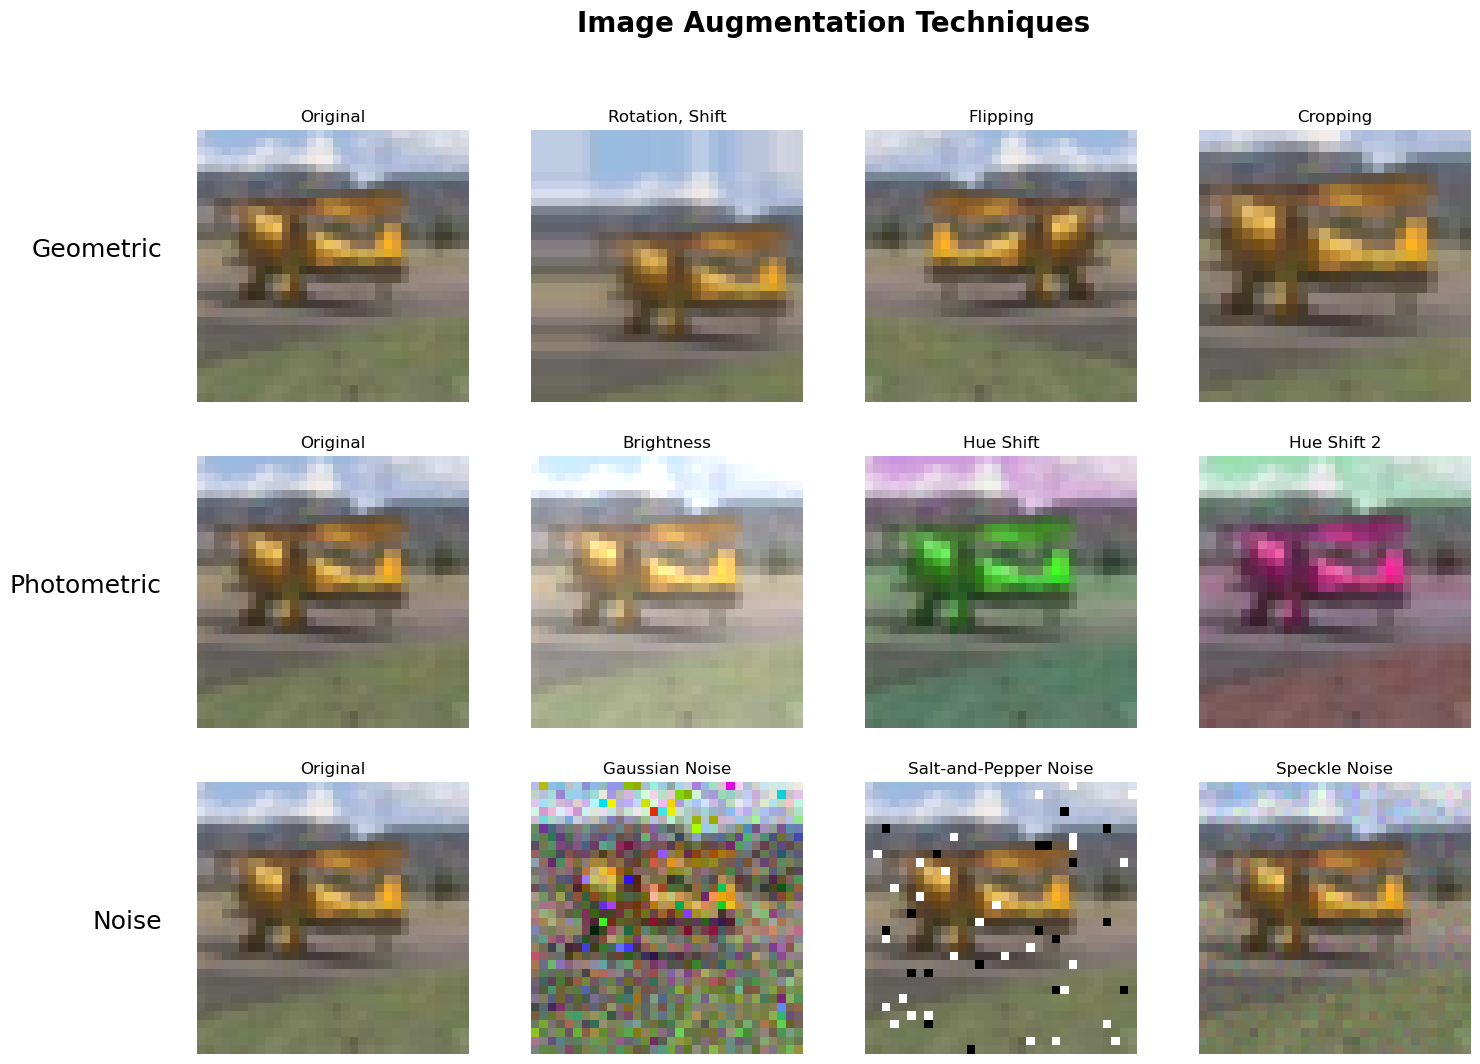
\includegraphics[width=.9\textwidth]{abb/traditional_image_augmentation_examples.png}
    \caption{Exemplary use of traditional augmentation techniques from the categories \textit{geometric} (first row), \textit{photometric} (second row), and \textit{noise-corruption} (third row). The image shown is an image from the \hyperref[used_datasets]{CIFAR10 dataset}, assigned to the class "airplane".}
    \label{fig:figure_tda_examples}
\end{figure}

\noindent
When applying the augmentations shown in Figure~\ref{fig:figure_tda_examples}, it is mandatory to consider domain-specific knowledge and constraints. For example, flipping images from the MNIST dataset to train a generative model may result in an image where a horizontally flipped "9" appears, which, in the domain of Arabic numerals, is semantically incorrect. Conversely, when classifying an airplane, which can have varying shapes, colors, three-dimensional orientations in space, and images taken through a dusted lens, applying all of the above augmentations could be beneficial.


\subsubsection[Generative Data Augmentation - GDA]{Generative Data Augmentation}\label{theoretical_gda}
Differing from the previously mentioned TDA \ref{theoretical_tda}, GDA does not focus on altering existing data instances but rather on creating entirely new samples that match the underlying data distribution of the training data. These generated instances may or may not include labels.

The goal is to train a generative model \( G \) that produces instances \( X_1 \), for example, from a noise vector \( z \), such that the distribution of the generated data approximates the true distribution \( P(X) \) of the original dataset. In this context, \( G \) can be viewed as a function:

\[
G: z \mapsto X_1, \quad X_1 \sim P_G(X) \approx P(X),
\]

\noindent
where \( P_G(X) \) is the learned distribution of the generative model, aiming to approximate the real data distribution \( P(X) \).

In the case of \textit{conditional} generative data augmentation, additional information such as class labels \( y \) is incorporated into the generation process. This allows the model to generate samples corresponding to specific categories within the data. The conditional generative model \( G \) then follows:

\[
G: (z, y) \mapsto X_1, \quad X_1 \sim P_G(X \mid y) \approx P(X \mid y),
\]

\noindent
where \( P_G(X \mid y) \) represents the learned conditional distribution, aiming to approximate the real class-conditioned data distribution \( P(X \mid y) \). This enables targeted data generation for specific categories, enhancing data diversity while maintaining class consistency.

% ########################################################################################################
% # END: DATA AUGMENTATION
% ########################################################################################################



% ########################################################################################################
% # START: Generative Aderserial Networks
% ########################################################################################################

\subsection[Generative Adversarial Network - GAN]{Generative Adversarial Network}\label{theoretical_gan}
Generative Adversarial Network (GANs) have first been introduced by Goodfellow at al. in 2014 \cite{goodfellow2014generativeadversarialnetworks} GANs are a type of generative models designed to learn the underlying data distribution of their training data and generate new, realistic instances. The core idea of the framework is an adversarial training process between two NNs: the textit{Generator} \(G\) and the \textit{Discriminator} \(D\), competing against one another in a minimax game \cite{VonNeumann1928Minimax}. The following figure (\ref{fig:figure_gan_arch}) shows a visualization of the vanilla gan architecture.

% TODO: inconsistencies between text and image rega
\begin{figure}[htbp]
    \centering
    \vspace{-4em}
    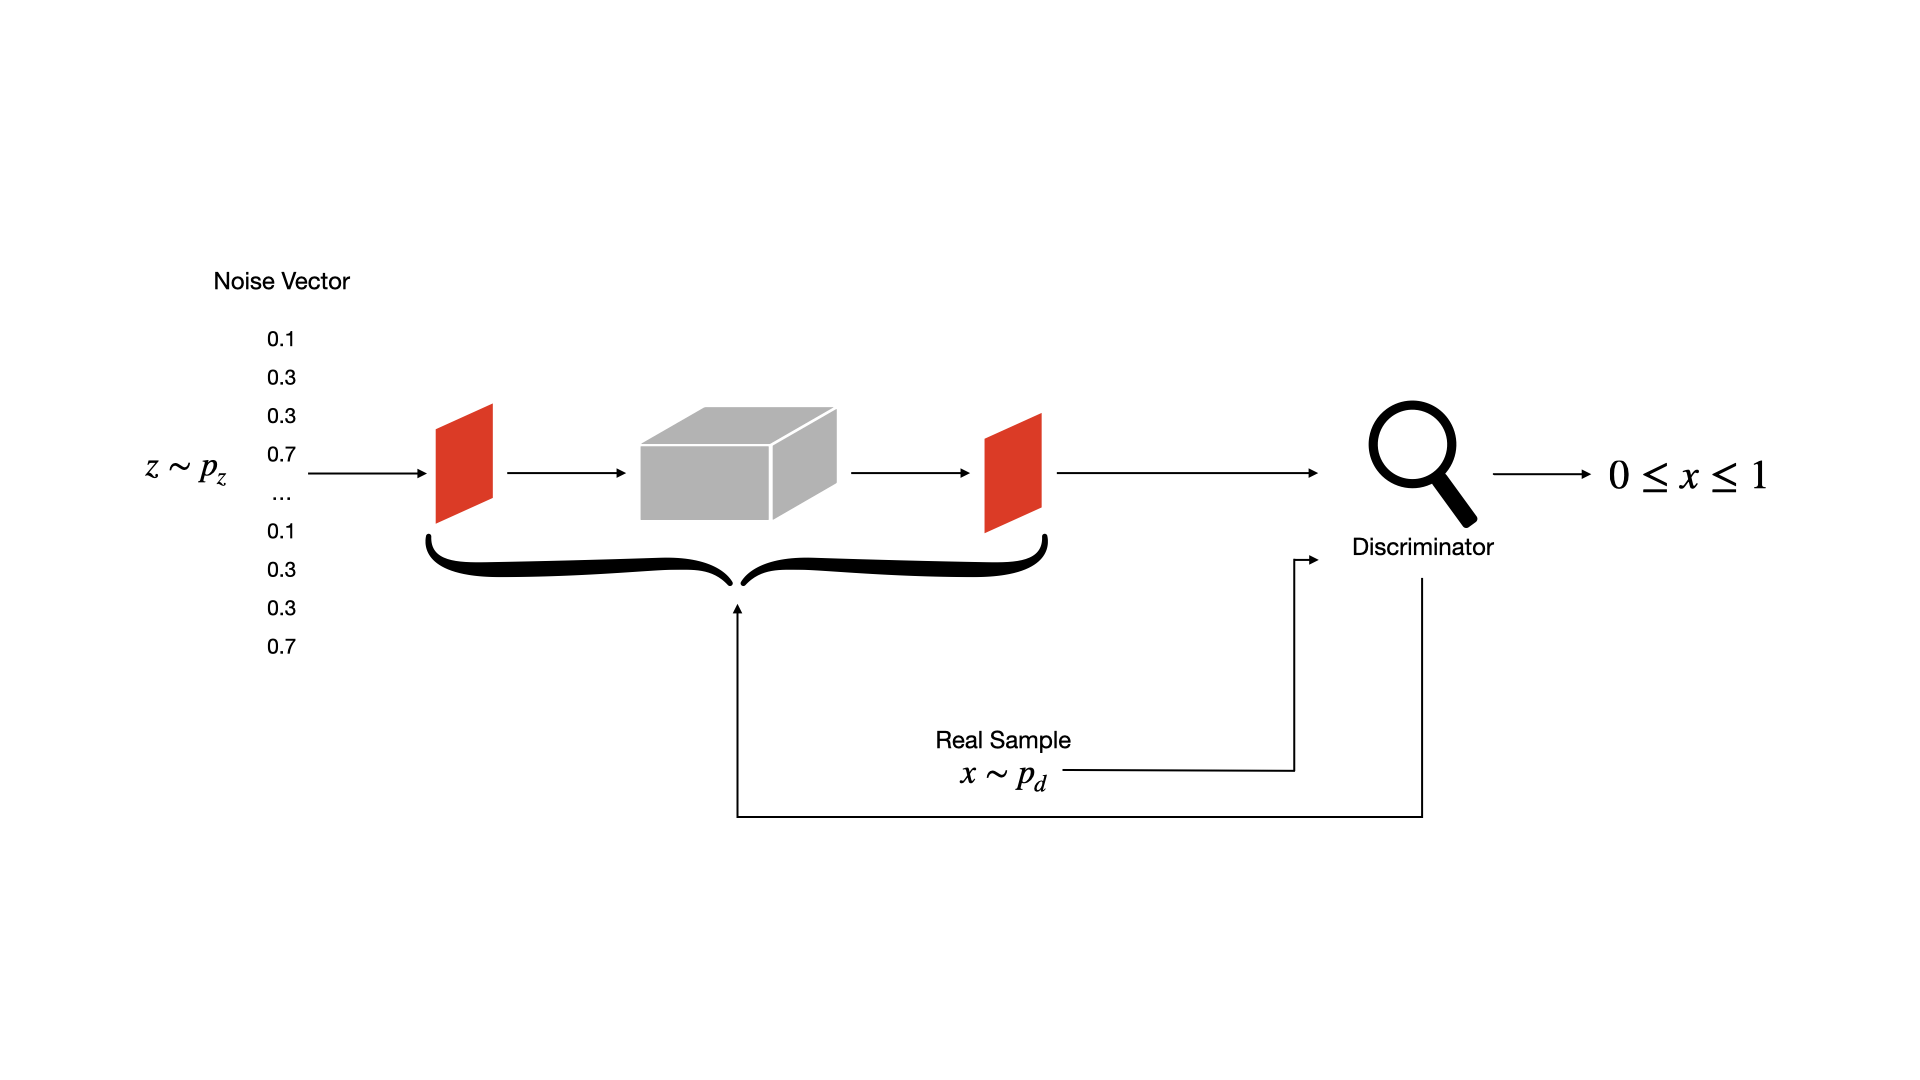
\includegraphics[width=.9\textwidth]{abb/arch_gan.png}
    \caption{Visualization of the vanilla GAN architecture. The figure shows the noise vector, flowing into the discriminator, as well as the real sample from \(P_d\)}
    \label{fig:figure_gan_arch}
\end{figure}


\subsubsection{Mathematical Formulation}\label{theoretical_gan_math}
Let \(X \sim P_{data}\) be samples drawn from the real data distribution, and let \(z \sim P_z\) be random noise sampled from a known prior (e.g., a Gaussian or uniform distribution). The generator \(G\) is a function \(G: \mathbb{R}^d \to \mathbb{R}^n\) that maps a noise vector \(z\) to a synthetic data instance \(\tilde{X}\), attempting to approximate \(P_{data}\):\(\tilde{X} = G(z), \quad z \sim P_z.\)

The discriminator \(D\) is a function \(D: \mathbb{R}^n \to [0,1]\) that outputs the probability that a given sample is real rather than generated. It is trained to distinguish between real samples \(X \sim P_{data}\) and generated samples \(\tilde{X} \sim P_G\), where \(P_G\) is the implicit distribution induced by \(G\).

The training objective is formulated as the following minimax game:

    \begin{equation}\label{theory_gan_vanilla_formula}
        \min_G \max_D \mathbb{E}_{X \sim P_{data}} [\log D(X)] + \mathbb{E}_{z \sim P_z} [\log (1 - D(G(z)))].
    \end{equation}

Here, the discriminator \(D\) aims to maximize the probability of correctly classifying real and fake samples, while the generator \(G\) aims to generate samples that fool \(D\), minimizing \(\log(1 - D(G(z)))\). In an ideal scenario, the game converges to a Nash equilibrium where \(G\) produces samples indistinguishable from real data, i.e., \(P_G \approx P_{data}\).

\subsubsection{Training Process}\label{theoretical_gan_training}
GAN training follows an alternating optimization approach:
\begin{enumerate}
    \item Update \(D\): Given a batch of real samples from \(P_{data}\) and fake samples generated by \(G\), update \(D\) to maximize its ability to discriminate real from fake data.
    \item Update \(G\): Generate new fake samples and update \(G\) to minimize \\ \(\log(1 - D(G(z)))\), effectively pushing \(G\) to generate more realistic samples.
    \item Repeat the process iteratively, typically using stochastic gradient descent (SGD) or Adam optimization.
\end{enumerate}

\subsubsection{Challenges in GAN Training}\label{theory_gan_problems}
Following, challenges that can occur during the training of gans are discussed. These have already been mentioned in the introductionary section \ref{problems_of_gans}. Here, they are described in greater detail.
\paragraph[Mode Collapse]{Mode Collapse}
Mode collapse occurs when the generator produces only a small subset of the data distribution, leading to a lack of diversity. Instead of generating varied samples, it repeatedly produces similar ones that fool the discriminator. This happens when the generator finds an easy "shortcut" rather than learning the full distribution. More formally, \(G\) collapses many values of \(z\) to the same value of \(x\) \cite{goodfellow2014generativeadversarialnetworks}. A common technique to mitigate this issue is  minibatch discrimination \cite{salimans2016improvedtechniquestraininggans}. In several studies, experiments have been conducted to enhance diversity of GANs (\cite{Chang2024QDGenSampling}, \cite{Humayun2021MaGNET}, \cite{Humayun2022PolaritySampling}) % TODO: I tried minibatch discrimination for the cifar madgan, but did not work
\paragraph[Lack of Inter-Class Diversity]{Lack of Inter-Class Diversity}
Even if mode collapse is avoided, GANs may struggle to generate samples that represent all data classes equally. This is a common issue in class-conditional GANs, where samples across different classes may overlap or lack distinct features. Causes include imbalanced datasets, poor class conditioning, or weak discriminator feedback \cite{Odena201710.5555/3305890.3305954}.
\paragraph[Failure to Converge]{Failure to Converge}
Unlike traditional neural networks, GANs follow an adversarial training process, making optimization highly unstable. The loss functions of both the generator and discriminator change dynamically, often leading to non-convergent behavior. Methods like Wasserstein GANs (WGAN) \cite{arjovsky2017wassersteingan} and spectral normalization \cite{miyato2018spectralnormalizationgenerativeadversarial} improve stability and help achieve better convergence.
\paragraph[Vanishing & unstable Gradients]{Vanishing \& unstable Gradients}
When the discriminator becomes too strong, it perfectly distinguishes real from fake samples, leading to vanishing gradients for the generator. This prevents meaningful updates, stalling progress. On the other hand, unstable gradients cause erratic updates, preventing smooth learning. Alternative loss functions (e.g., LSGANs \cite{mao2017squaresgenerativeadversarialnetworks}) and spectral normalization help stabilize training.
\paragraph[Imbalance between Generator and Discriminator]{Imbalance between Generator and Discriminator}
A well-balanced GAN requires both models to improve at a similar pace. If the discriminator overpowers the generator, training halts. If it's too weak, the generator receives poor feedback and produces low-quality outputs \cite{goodfellow2014generativeadversarialnetworks}. Balancing techniques include adaptive learning rates, gradient penalties, and label smoothing \cite{Radford2015DCGAN}.


\subsection[Deep Convolutional Generative Adversarial Network - DCGAN]{Deep Convolutional Generative Adversarial Network}\label{theoretical_dcgan}
Deep Convolutional Generative Adversarial Networks (DCGANs) were introduced by Radford et al. in 2015 \cite{Radford2015DCGAN} as an improvement over vanilla GANs. While the fundamental adversarial framework remains the same (see \hyperref[theoretical_gan_math]{3.3 Mathematical Formulation}, \hyperref[theoretical_gan_training]{3.3 Training Procecss}), DCGANs leverage deep convolutional neural networks to enhance stability and generate higher-quality images.

\subsubsection{Architectural Adjustments}\label{theorey_dcgan_architecture}
To improve training stability and image quality, DCGANs implement the use of \hyperref[theoretical_classification_conv_layers]{convolutional layers}.

\begin{itemize}
    \item \textbf{Convolutional Architecture:} Fully connected layers in both \(G\) and \(D\) are replaced with deep convolutional layers, enabling better spatial feature extraction.
    \item \textbf{Strided Convolutions:} In the discriminator, pooling layers are removed in favor of strided convolutions, reducing the risk of information loss.
    \item \textbf{Transposed Convolutions:} The generator employs transposed convolutions (also known as fractionally-strided convolutions) instead of upsampling layers to improve the quality of generated images.
    \item \textbf{Batch Normalization:} Applied to both \(G\) and \(D\), batchnorm helps stabilize training by reducing internal covariate shift \ref{theoretical_classification_batchnorm_layers}. Batchnorm is omitted in the generator’s final layer to allow unrestricted output variability and in the discriminator’s input layer to preserve the original data distribution.
    \item \textbf{LeakyReLU Activation:} The discriminator uses LeakyReLU instead of standard ReLU to prevent dying neurons and allow gradients to flow through negative inputs \ref{theoretical_activations_leakyrelu}.
    \item \textbf{No Fully Connected Layers:} Fully connected layers are removed to maintain spatial coherence in generated images, as they discard spatial information by flattening feature maps. Instead, convolutional layers preserve local structures, enabling more realistic image synthesis \ref{theoretical_classification_fully_connected_layers}.
\end{itemize}


\subsection[Conditional Generative Adversarial Network - cGAN]{Conditional Generative Adversarial Network}\label{theoretical_cgan}

Conditional Generative Adversarial Networks (cGANs), introduced by Mirza and Osindero in 2014 \cite{mirza2014conditionalgenerativeadversarialnets}, extend the vanilla GAN framework by incorporating additional information \(y\), such as class labels, into both the generator and discriminator. This allows cGANs to generate samples conditioned on specific attributes, enabling controlled generation.

\subsubsection{Mathematical Formulation}
\label{theoretical_cgan_math}
The core idea of cGANs is to condition both the generator \(G\) and the discriminator \(D\) on auxiliary information \(y\). Instead of generating data solely from a noise vector \(z\), the generator now takes \(y\) as an additional input:

\begin{equation}
\tilde{X} = G(z, y)
\end{equation}

\noindent
Similarly, the discriminator receives both the real or generated sample and the corresponding condition:

\begin{equation}
D(X, y) \quad \text{and} \quad D(G(z, y), y)
\end{equation}

\noindent
The adversarial objective function for cGANs extends the standard GAN loss to incorporate this conditional dependency:

\begin{equation}\label{theory_gan_cond_formula}
\min_G \max_D \mathbb{E}_{X, y \sim P_{data}} [\log D(X, y)] + \mathbb{E}_{z \sim P_z, y \sim P_y} [\log (1 - D(G(z, y), y))]
\end{equation}

\noindent
This formulation forces to generate samples that align with the given condition , while  learns to discriminate between real and generated samples, considering their respective conditions.

\subsubsection{Architectural Adjustments}
\label{theory_cgan_architecture}
To implement cGANs, architectural adjustments are necessary compared to vanilla GANs:

\begin{itemize}
    \item \textbf{Input Conditioning:} Both the generator and discriminator must receive the conditional information y as input. This is typically achieved by concatenating the condition y with the noise vector z in the generator's input and with the input image X in the discriminator's input.
    \item \textbf{Embedding Conditional Information:} For categorical conditions (e.g., class labels), the condition y is often embedded into a lower-dimensional vector before concatenation. This embedding allows the network to learn meaningful representations of the conditions.
    \item \textbf{Concatenation, Addition, or Multiplication:} The conditional information can be incorporated through concatenation, addition, or element-wise multiplication at various layers within the generator and discriminator, depending on the specific application and architecture.
    \item \textbf{Preservation of Conditional Information:} Care must be taken, that the conditional information is preserved throughout the network. This means, that the information must traverse the network, all the way to the output layer.
\end{itemize}

These architectural modifications ensure that the generator and discriminator can effectively utilize the conditional information to generate and discriminate samples based on the given conditions.

\subsection[Multi-Agent Diverse Generative Adversarial Network - MADGAN]{Multi-Agent Diverse Generative Adversarial Network}
\label{theoretical_madgan}
MADGAN is proposed as a generalized framework for the GAN architecture \cite{ghosh2018madgan}. The framework employs multiple generators, one discriminator and an adjusted objective for the discriminator. The adjusted objective aims to enforce the identifications of the generator creating given fake images. These changes specifically aim to ease the first two mentioned problems of GANs, namely \textit{Mode Collapse} and \textit{Lack of Inter-Class Diversity} \ref{theory_gan_problems}. This chapter delves into the specifics of this framework: integetration of multi-agent systems with diversity-promoting techniques, within the GAN framework. The following subsections will detail the architecture, objective function, and training procedure of the MADGAN framework.

\begin{figure}[htbp]
    \centering
    \vspace{-4em}
    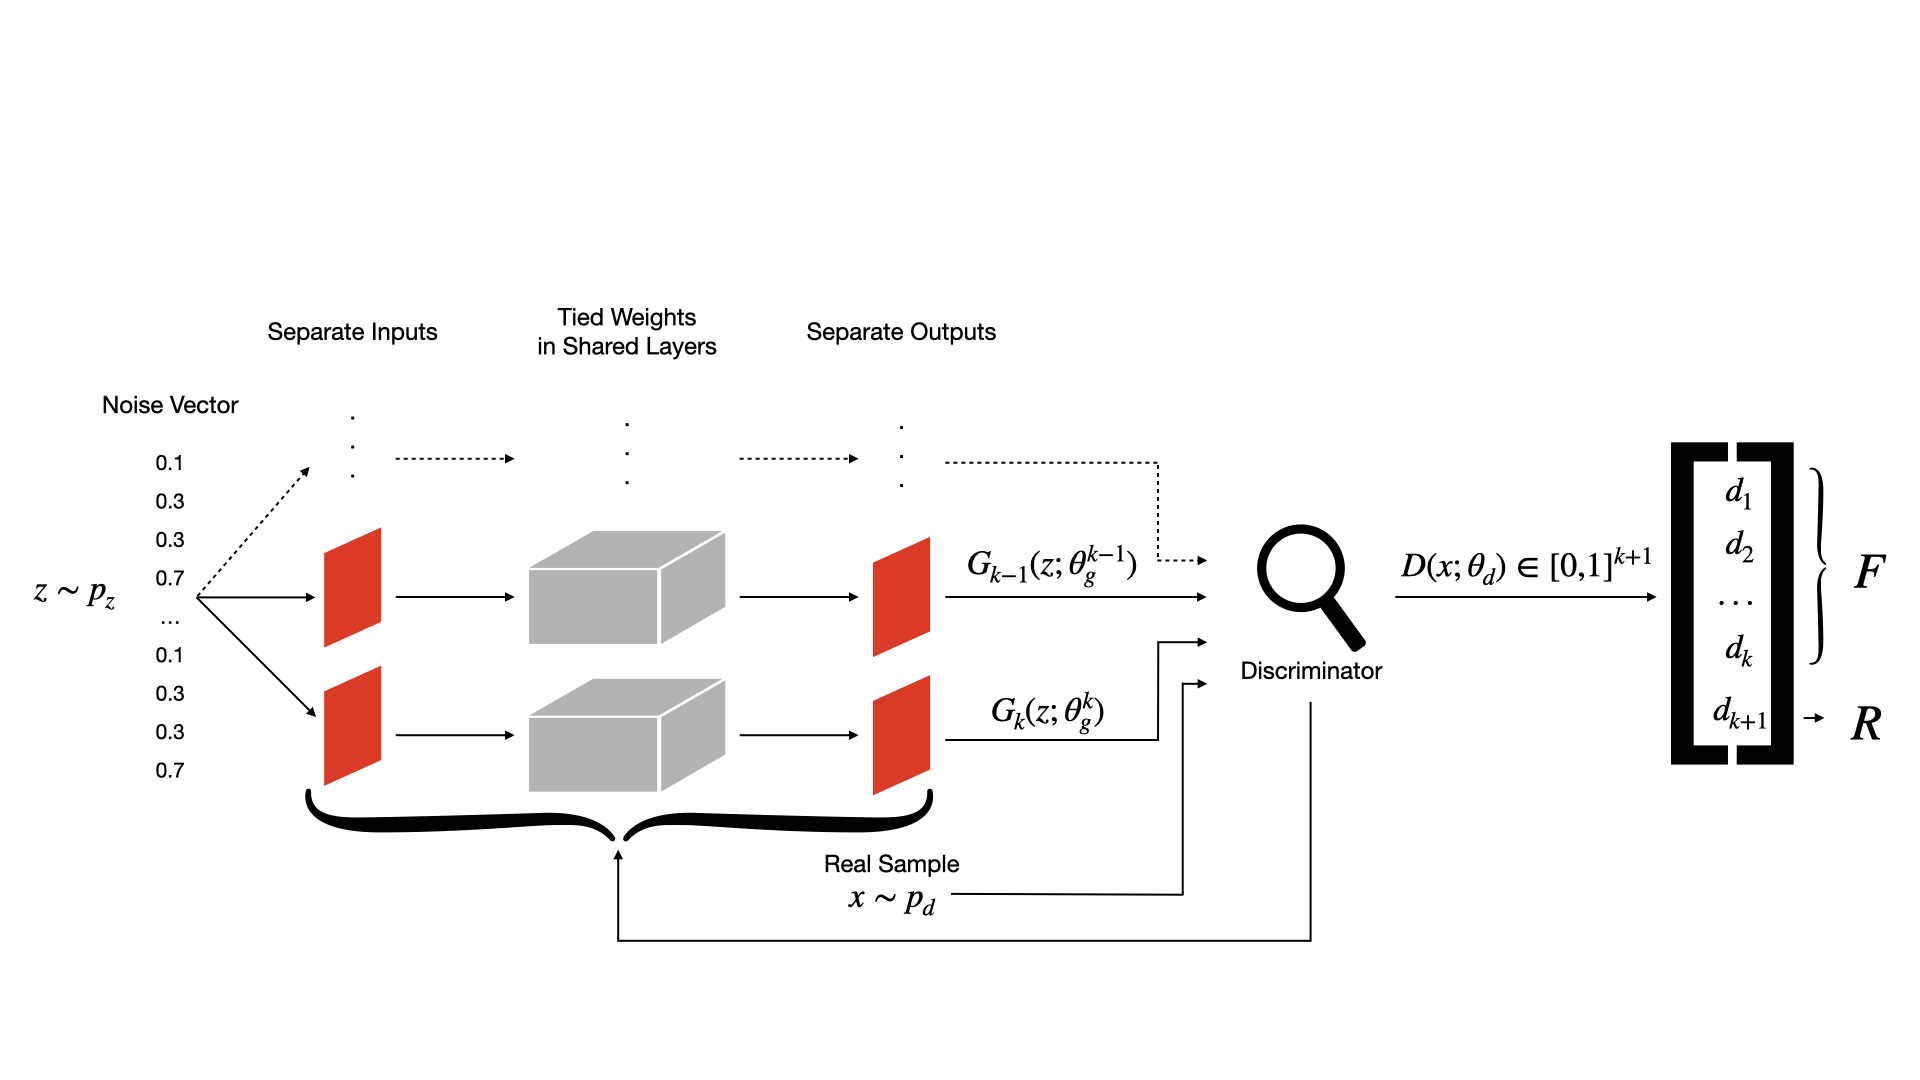
\includegraphics[width=.9\textwidth]{abb/arch_madgan.png}
    \caption{Visualization of the MADGAN architecture. The figure shows the \(k+1\) outputs of the discriminator and the \(k\) generators, with tied weights in the middle of the network.}
    \label{fig:figure_madgan_arch}
\end{figure}


\subsubsection{Mathematical Formulation}
\label{theoretical_madgan_math}
As afore mentioned, the MADGAN architecture employs multiple generators and one discriminator. The goal the for \(K\) generators is to generate samples from different high probability regions of the data \(P_{data}\). In order to guide the generators into their respective direction, the objective of the discriminator has been modified, in which it no longer has to just differentiate between real and fake images, but also identify the generator that produced a given fake instance. Intuitively, the discriminator thereby forces the generators into mostly disjoint regions within the real data distribution. Inspired by the formulation for the discriminator in the paper "\textit{Improved Techniques for Training GANs}" \cite{salimans2016improvedtechniquestraininggans}, their discriminator model has an output of \(k+1\), utilizing the \textit{Softmax} activation function \ref{theoretical_activations_softmax}, where \(k\) sets the number of used generators. The output at \(k+1\) represents the probability that the given samples belongs to the real data distribution \(P_{data}\), whereas the scores at \(j \in \{ 1, ..., k \}\) describe the probability of said sample originating from either of the generators. The above figure \ref{fig:figure_madgan_arch} shows a visualization of the architecture. Thus, when learning the discriminators parameters \(\theta_d\), the cross-entropy between the softmax outputs and the \textit{Dirac delta distribution} (Ddd) \(\delta \in \{0, 1\}^{k+1}\) is optimized. Here, \(\delta(j) = 1\) is 1, if the sample belongs to the \(j\)-th generator, else \(\delta(k+1) = 1\) if the sample originates from \(P_{data}\). Following this definition, the Ddd \(\delta\) can be understood as a one-hot encoding indicating whether a given sample is real of, and if not, from which generator it originates
\footnote{It is important to point out, that the Dirac delta distribution is actually continuous. Their usage of the Ddd reminds of the Kronecker delta function, which \( \delta(i,j) = 1 \text{ for } i=j; 0 \text{ for } i \ne j \).}
. The objective function for the optimization of \(\theta_d\), with \(\theta_g\) freezed is therefore:
\begin{equation}
    \max\limits_{\theta_d}\mathbb{E}_{x \sim p} H(\delta, D(x; \theta_d))
\end{equation}

\noindent
\(H(...)\) here represents the negative cross-entropy function. Important to piont out here is that, "Intuitively, in order to correctly identify the generator that produced a given fake sample, the discriminator must learn to push different generators towards different identifiable modes." \cite{ghosh2018madgan}, page 4. \hyperref[fig:figure_madgan_diverse_mode_push]{Figure 2} shows a visualization of the generators being pushed to diffenret modes. The objective for the generators however, remains semantically the same as in the vanilla GAN \ref{theory_gan_vanilla_formula}. The difference here is that the objective function is generalized with an indexing \(i\) for the number of generators. That is, for the \(i\)-th generator, the objective function is to minimize:

\begin{equation}
    \mathbf{E}_{x \sim P_{data}} [ \log D(X; \theta_d) ] + \mathbf{E}_{z \sim P_{z}} \log (1-D_{k+1}(G_i(z; \theta_{g}^{i}); \theta_x))
\end{equation}

\textbf{Enforing Diverse Modes:}
The researchers provide a theorem demonstrating that the \(k\) generators collectively form a mixture model. In it, each generator represents a mixture compotonent to the global optimimum of \( -(k+1)\log(k+1)+1 \log k \). This is achieved, when \(p_{data} = \frac{1}{k}\sum_{i=1}^{k} p_{g_i}\). It is to point out that, for \(k = 1\), the case with one generator, one obtains the exact Jensen-Shannon divergence based objective, as shown in the vanilla GAN paper by Goodfellow et al. \cite{goodfellow2014generativeadversarialnetworks}. Following their proof, the objective function for all \(k\) generators is to minimize:

\begin{equation}
    \mathbf{E}_{x \sim P_{data}} [ \log D_{k+1}(X) ] + \sum_{i=1}^{k}\mathbf{E}_{x \sim p_{g_i}} \log (1-D_{k+1}(x))
\end{equation}

\noindent
The exact formulation of their theorem, proof and propositions can be found in Ghosh et al. \cite{ghosh2018madgan}, following formulas (3) through (9).

\begin{figure}[htbp]
    \centering
    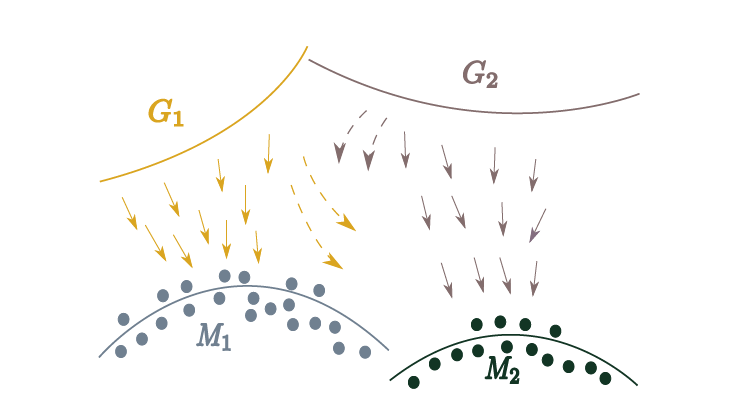
\includegraphics[width=.9\textwidth]{abb/madgan_diverse_mode_push.PNG}
    \caption{Figre taken from the original paper \cite{ghosh2018madgan}. The visualization shows how different generators \(G_1\) and \(G_2\) are pushed to different modes \(M_1\) and \(M_2\)}
    \label{fig:figure_madgan_diverse_mode_push}
\end{figure}

\subsubsection{Architectural Adjustments}
\label{theory_madgan_architecture}
The architecture changes can be summarized into three mayor changes applied to the vanilla GAN (\ref{theoretical_gan}) architecture:

\noindent\textbf{Multiple Generators:} The MADGAN architecture employs multiple generators instead of a single one. Following the intuition behind the adjusted disciminator objective, the respective gans distribute into different, mostly disjoint regions in the real data distribution.

\noindent\textbf{Modified Discriminator Objective:} The discriminator in this architecture outputs \(k + 1\) instead of \(1\) utilizing the softmax function \ref{theoretical_activations_softmax}. One output for every generator indicating wheter an image originates from either one of the generator and one output implying if the discriminator cam to the conclusion that the current image is fake or not. As afore described, this ecurages the discriminator to push the generators into identifiable distinct outptus.

\noindent\textbf{Parameter Sharing among Generators:} Generators in the MADGAN architecture share most of their layers between the \(k\) generators. This reducese redundant compute in the initial feature extraction layers capturing high-frequency structures common in many datasets. Especially in single-view data, this is recommended. For multi-view data it is not recommended, to allow each generator to capture mode-specific features.

% ########################################################################################################
% # END: Generative Aderserial Networks
% ########################################################################################################


% ########################################################################################################
% # START: Image Scores
% ########################################################################################################

\subsection{Image Scores}\label{theoretical_image_scores}

To quantitatively evaluate the quality and diversity of images generated by generative models, several metrics have been proposed in the literature. These image scores aim to provide an objective measure to compare generative models independently of human evaluation. This section introduces widely-used metrics for evaluating generative models: \textit{Inception Score} (IS), \textit{Fréchet Inception Distance} (FID), and the underlying InceptionV3 model employed for these metrics.

\subsubsection[Inception Score - IS]{Inception Score}
The Inception Score (IS) \cite{salimans2016improvedtechniquestraininggans} is one of the earliest and most commonly used metrics for evaluating generative models, especially GANs. It leverages a pretrained InceptionV3 classifier to assess two main criteria of generated images:

\begin{itemize}
    \item \textbf{Image Quality (Objectiveness)}: Each generated image should be classified into a specific class with high confidence. This corresponds to a low-entropy conditional label distribution \( p(y|x) \).
    \item \textbf{Diversity}: Across the entire set of generated images, the distribution of predicted classes should be diverse and cover many different labels. This corresponds to a high-entropy marginal label distribution \( p(y) \).
\end{itemize}

Mathematically, the Inception Score is computed as:
% TODO: check them formulas
\begin{equation}
IS = \exp \left( \mathbb{E}_{x \sim p_g} \left[ D_{\text{KL}}(p(y|x) \| p(y)) \right] \right)
\end{equation}

where \( D_{\text{KL}} \) denotes the Kullback-Leibler divergence between the conditional class distribution and the marginal class distribution.

\textbf{Limitations of IS}:
\begin{itemize}
    \item Does not directly compare generated images with real images.
    \item Insensitive to intra-class diversity.
    \item Sensitive to the choice of the pretrained classifier.
\end{itemize}

\subsubsection[Fréchet Inception Distance - FID]{Fréchet Inception Distance}

The Fréchet Inception Distance (FID) \cite{heusel2018ganstrainedtimescaleupdate} improves upon IS by directly comparing the feature distributions of real and generated images. FID embeds both real and generated images into a lower-dimensional feature space (obtained from a pretrained InceptionV3 network) and models these embeddings as multivariate Gaussians.

Let \( (\mu_r, \Sigma_r) \) and \( (\mu_g, \Sigma_g) \) denote the means and covariances of the real and generated image features, respectively. The FID score is computed as:
% TODO: check them formulas
\begin{equation}
FID = \| \mu_r - \mu_g \|^2_2 + \text{Tr} \left( \Sigma_r + \Sigma_g - 2(\Sigma_r \Sigma_g)^{1/2} \right)
\end{equation}

\textbf{Interpretation}:
\begin{itemize}
    \item Lower FID indicates better quality and diversity.
    \item Sensitive to both image quality and intra-class diversity.
\end{itemize}

\textbf{Advantages over IS}:
\begin{itemize}
    \item Considers real image distribution.
    \item Sensitive to intra-class mode collapse.
\end{itemize}

\textbf{Limitations}:
\begin{itemize}
    \item Assumes Gaussian distribution of features.
    \item Sensitive to the choice of feature extractor.
\end{itemize}

\subsubsection[InceptionV3 Model]{InceptionV3 for Image Evaluation}

Both IS and FID rely on the InceptionV3 model~\cite{szegedy2016rethinking}, a deep convolutional neural network trained on ImageNet. The InceptionV3 network serves two primary roles in generative image evaluation:

\begin{enumerate}
    \item \textbf{Feature Extractor}: Intermediate activations (typically from the pool3 layer) are used as a semantic representation of the images for computing FID.
    \item \textbf{Classifier}: The output class probabilities of InceptionV3 are used to compute IS.
\end{enumerate}

\textbf{Properties of InceptionV3 relevant for image scoring}:
\begin{itemize}
    \item Trained on large-scale ImageNet dataset — providing a rich semantic feature space.
    \item Fixed, non-trainable weights during evaluation — ensuring standardization.
    \item Layer choice affects sensitivity — earlier layers capture texture, later layers capture semantics.
\end{itemize}

\textbf{Limitations of using InceptionV3}:
\begin{itemize}
    \item Domain gap between ImageNet images and domain-specific generative tasks (e.g., medical images, industrial images).
    \item Performance can degrade if generated images differ significantly from ImageNet classes.
\end{itemize}


% ########################################################################################################
% # STOP: Image Scores
% ########################################################################################################









\newpage
